\documentclass[../Bachelorarbeit.tex]{subfiles}

\begin{document}
\label{sec:VBS}

Vector Boson Scattering (\acrshort{vbs})\cite{Bittrich.27.05.2020} refers to the scattering of any electroweak gauge Boson V=$W^{\pm}$, Z, $\gamma$. This
definition includes diboson processes which makes it necessary to specify the final state for \acrshort{vbs} and diboson processes.
The \acrshort{vbs} finale state $VVjj$ is characterized by the two bosons and two jets while diboson processes finale state only contains
two bosons $VV$ in the finale state. Since gauge bosons have a short half-life of $3 \cdot 10^{-25}$s one needs to include the
decay of the outgoing boson leading to the full process $qq\rightarrow VVjj\rightarrow 4ljj$ shown in figure \ref{fig:feynman_full_VBS}.
\begin{figure}[h]
    \centering
    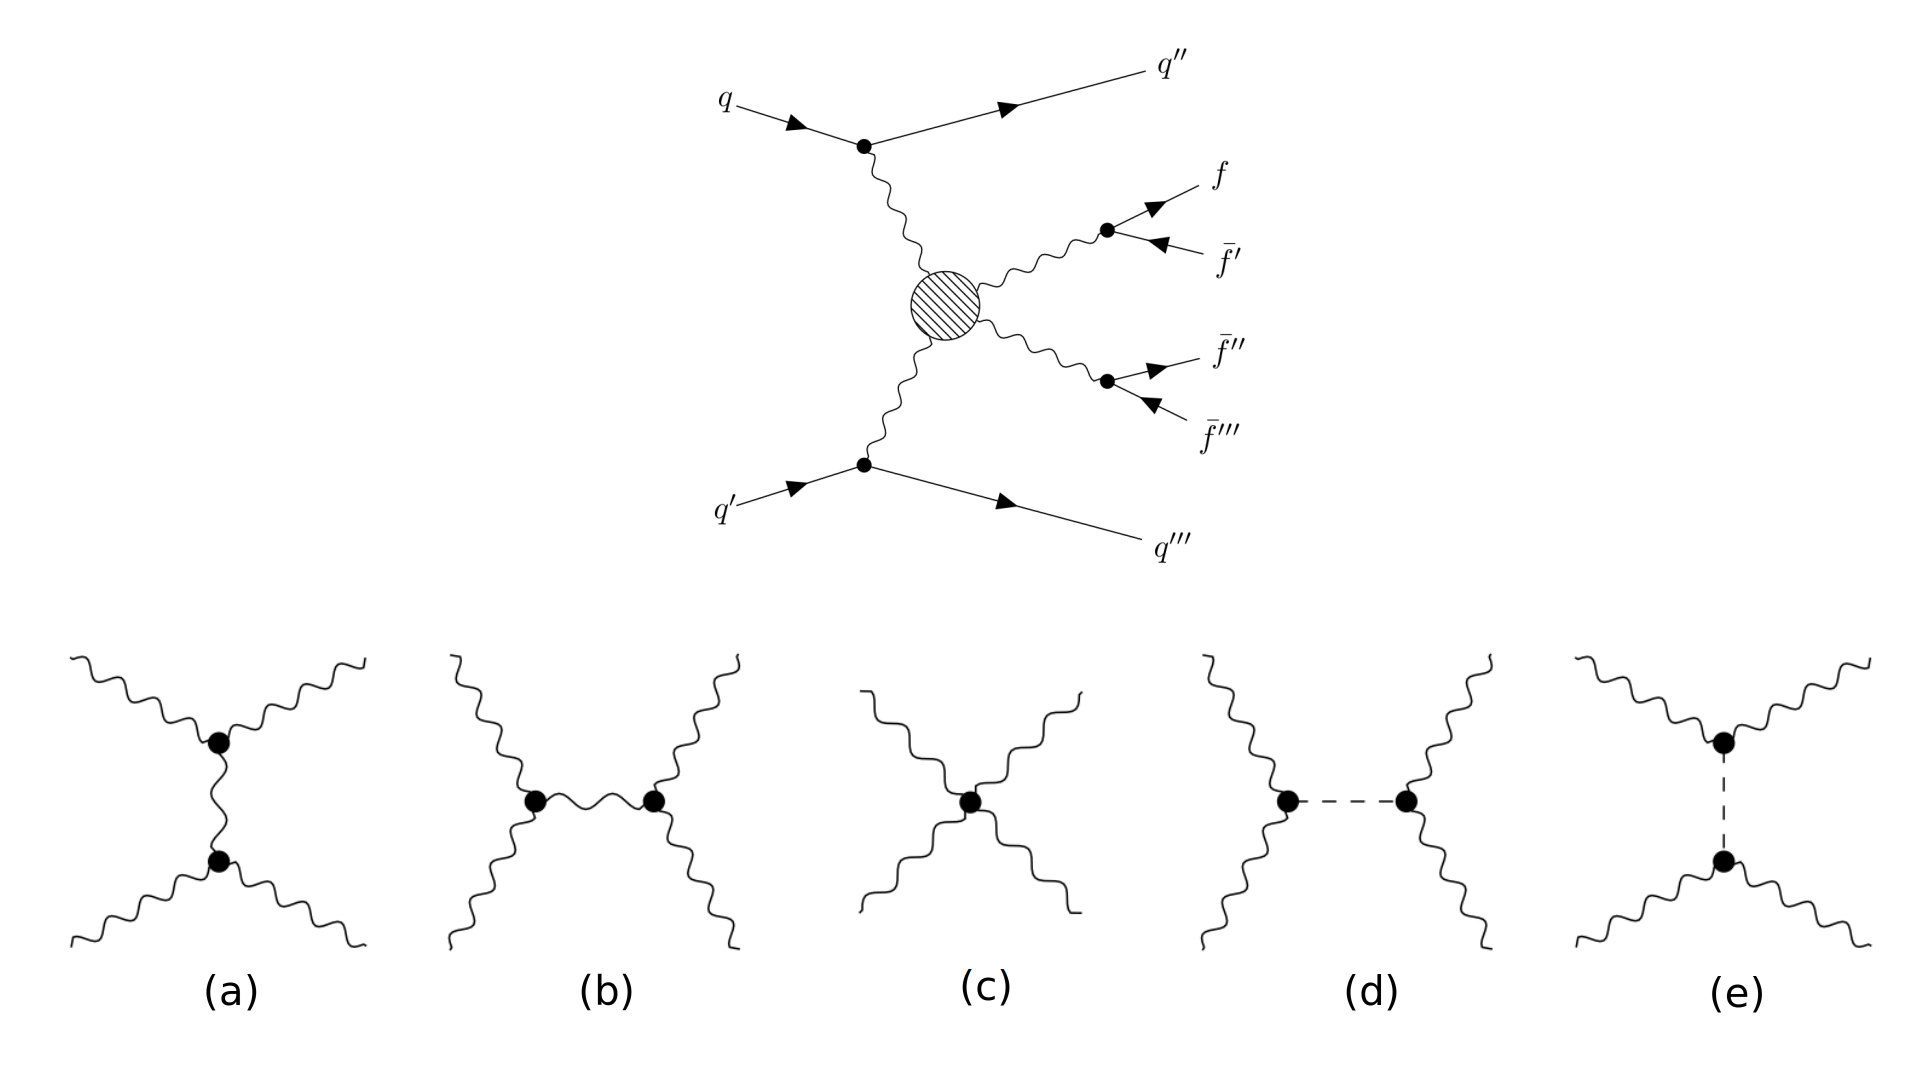
\includegraphics[width=\textwidth]{images/feynman_full_VBS.png}
    \caption{Structure of full \acrshort{vbs} process $qq\rightarrow VVjj\rightarrow 4ljj$ with two of the four leptons having a charge. The circle stands for the processes a to e
        which come from the non-Albanian gauge group $SU(2)$ for weak interactions in leading order $VV \rightarrow VV$ processes.\cite{Bittrich.27.05.2020}}
    \label{fig:feynman_full_VBS}
\end{figure}
In leading order only quark-initiated diagrams produce vector bosons. These quarks are shifted by a small angle away from
the beam axis resulting in the for the \acrshort{vbs} process characteristic tagging jets. The couplings a to e in \ref{fig:feynman_full_VBS}
are all electroweak interactions and based on there coupling structure produce a squared matrix element
$\left\lvert M^{2} \right\rvert \propto \alpha_{EW}^{6}$. The $\alpha_{EW}$ stands for the combined coupling strength of
the electroweak and electromagnetic interactions. These couplings can also be achieved by coupling structure
$\left\lvert M^{2} \right\rvert \propto \alpha_{EW}^{4}\alpha_{S}^{2}$, but these couplings however do not contribute to \acrshort{vbs} processes.
In the signal for \acrshort{vbs} processes the diagrams with less than six electroweak diagrams are considered as background defining the $VVjj-EW6$ processes.
Some examples for the these processes can be seen in \ref{fig:EW6}. How these processes are selected will be discussed in the following chapter.
The $W^{\pm}Z$ processes is dominated by EW and QCD interactions specifically the \acrshort{eft} Terms are only accounted for in the EW interactions.\\\\
\begin{figure}[h]
    \centering
    \includegraphics[width=\textwidth]{images/EW6.png}
    \caption{Example Feynman diagrams for VVjj-EW6 processes. The dashed circle stands for the Feynman diagrams a-e in Figure \ref*{fig:feynman_full_VBS}}
    \label{fig:EW6}
\end{figure}
Multiple factors make the study of \acrshort{vbs} processes interesting. \acrshort{vbs} processes are only accessible from \acrshort{lhc} Run-II and forward making them more relevant in the future.
The appearance of both \acrshort{tgc} and \acrshort{qgc} lead to interesting studies of polarization, gauge invariance, unitarity and Higgs physics.
The distinct two jet finale state makes the selection of \acrshort{vbs} process relatively easy leading to a small background estimation. In \acrshort{bsm} both properties
are relevant as new models often include \acrshort{tgc} and \acrshort{qgc}. Without knowing the underlying theory it is hard to make predictions on the impact of a \acrshort{bsm} theory on the background.
In \acrshort{eft} \acrshort{tgc} are essential for analysis on dim-6 operates and \acrshort{qgc} for studying dim-8 operators. The accessibility of a variety of couplings and
the fact that no \acrshort{bsm} theory to date fully describes anomalous couplings motivate the research on resonances in \acrshort{vbs} using \acrshort{eft}.


\end{document}
